\documentclass{article}
\usepackage[utf8]{inputenc}
\usepackage{tikz}
\usepackage{wrapfig}
\graphicspath{ {./} }

\begin{document}  
% main workflow




\centerline{\includegraphics[width=0.5\textwidth]{logo}}




\centerline{{\Large \textbf{Fakulta aplikovaných věd}}}
\centerline{{\Large \textbf{Západočeská univerzita v Plzni}}}



\centerline{{\Large \textbf{Semestrální práce KIV/PC}}}
\centerline{{\Large \textbf{Optimalizace funkce geneticým algoritmem}}}




\hspace*{\fill} \textbf{Ľubomír Bartoš \ (A16B0003P)}

\hspace*{\fill} \textbf{bartosl@students.zcu.cz}

\hspace*{\fill} \textbf{6. 1. 2019}



\newpage







\tableofcontents
\newpage

\section{Zadání}

Naprogramujte v ANSI C přenositelnou konzolovou aplikaci, která bude hledat extrém funkce

pomocí genetického algoritmu.

Genetický algoritmus je technika, která napodobuje procesy známé z biologie a hledá tak optimální

řešení zadaného problému. Podle zadaného problému se nadefinuje tzv. fitness funkce, jejíž

hodnota vyjadřuje životaschopnost potomka a vhodnost řešení problému.
\section{Základní princip genetického algoritmu:}
\begin{enumerate}
\item Náhodně vytvoříme několik různých řešení zadané úlohy a jedincù.
\item Provedeme křížení jedincù.
\item Náhodně zmutujeme malý počet jedinců.
\item Ověříme, jak dobře jeden každý jedinec řeší náš problém tak, že pro každého získáme hodnotu fitness funkce.
\item Vytvoříme novou generaci.
\item Opakujeme body 2 až 5. \ 
\end{enumerate}


\section{Úvod}

Semestrální práce obsahuje program, který dokáže ladit vstupní hodnoty programu a hledat tak extrém možného fitness ohodnocení. Program, který hodnotil tvořené vstupní hodnoty, byl při vývoji black box, k dispozici byl jen vstup/výstup programu, proto nevím zda nejlepší výsledky, které jsem pomocí svého algoritmu dosáhl, jsou opravdu extrémem. 



Má implementace se v několika ohledech odchyluje od zadání. Na funkčnost a správnost algoritmu by to nemělo mít vliv. Mutaci populace jsem v procesu posunul před tvoření potomků. V pokročilejších generacích by zmutovaní jedinci skoro nikdy nepřežili část umírání, protože by měli oproti zbytku malou fitness. Křížení binární části genu jsem implementoval tak, že se každý bit bere náhodně od matky nebo od otce, místo toho rozdělení genů na vhodném místě. Výběr jedinců k páření probíhá až po umírání slabých jedinců, navíc ze zbylých naprůměrných jedinců se bere jeden naprůměrný (z nadprůměrných) rodič a druhý náhodně pro mírné zvýšení zvýšení kvality populace.


\subsection{Konfigurace programu}

Program je konfigurovatelný pomocí tzv. metadata souboru, kde se definuje název, poměnné a parametry laděného programu. Počet jedinců v generaci nebyl blíže specifikován, vybral jsem tedy konstantní limit populace 100, definovanou v souboru structures.h. Při tvoření počáteční populace řešení a při plození potomků se vždy tvoří jedinci, dokud populace nedosáhne definovaného limitu.


\subsection{Formát souboru s metadaty}
\begin{itemize}
\item Na první řádce se nachází vždy spustitelný soubor s laděnou funkcí, který nám dává fitness pro jedince.
\item Následují data o konstantách a proměnných.
\begin{itemize}
\item Proměnná je definovaná na dvou řádcích. První řádek obsahuje informace o intervalu proměnné a o jejím typu. Na následujícím řádku se nachází název proměnné a nějaká konkrétní hodnota. Pouze tento typ řádku se v průběhu programu mění. Program momentálně umí pracovat s celočíselnou a reálnou proměnnou. 
\item Příklad reálné proměnné: \ 
\begin{itemize}
\item \#\_(10,18);R
\item a = 15.42069
\end{itemize}
\item Příklad celočíselné proměnné:
\begin{itemize}
\item \#\_(0,500);Z
\item c = 420
\end{itemize}
\item Konstanty mají formát jako proměnné, bez prvního řádku:
\begin{itemize}
\item b = 2
\end{itemize}
\end{itemize}
\item Prázdné řádky jsou ignorovány.
\end{itemize}


\section{Princip tohoto genetického algoritmu:}
\begin{enumerate}
\item Náhodně vytvoříme několik různých jedinců, obsahujících geny s řešením zadané úlohy.
\item Otestujeme geny jedinců a přiřadíme jim fitness (ohodnocení).
\item Jedince s podprůměrným fitness odstraníme.
\item Náhodně zmutujeme zadané procento populace (pokaždé u jedince jen jeden typ genu).
\item Doplníme generaci o potomky existujících jedinců (křížením vybraných rodičů).
\item Opakujeme body 2 až 5. \ 
\end{enumerate}


\subsection{Zdrojový soubor nature.c}

V tomto souboru souboru jsou definované zejména funkce simulující přírodní procesy přírody (vytvoření jedinců, množení, umírání, mutace, logika evoluce).


\subsection{Zdrojový soubor config.c}

V tomto zdrojovém souboru jsou definovány operace hledání nad seznamem populace, práce se soubory a laděnou funkcí, načtení konfigurace z metadata souboru.


\section{ \ Struktury a konstanty:}

Pro pojmenovávání struktur a funkcí jsem se snažil hledat slova podobná strukturám a procesům přírody. Strukt environment představuje "prostředí" , neboli konfiguraci pro vývoj jedinců. Obsahuje také názvy souborů a programů, které potřebujeme pro spuštění laděné funkce. Strukt creature představuje jedince, který nese gen s proměnnými vstupními hodnotami laděné funkce.
\subsection{Konstanty ve structures.h}
\begin{itemize}
\item VARIABLE\_TYPE\_INTEGER 'Z'
\begin{itemize}
\item typ proměnné z metadata souboru, představuje celé číslo
\end{itemize}
\item VARIABLE\_TYPE\_REAL 'R'
\begin{itemize}
\item typ proměnné z metadata souboru, představuje reálné číslo
\end{itemize}
\item POPULATION\_LIMIT 100
\begin{itemize}
\item limit populace
\end{itemize}
\item DEFAULT\_MUTATION\_RATE 5
\begin{itemize}
\item pokud není procento mutace populace zadáno z příkazové řádky, je nastaveno na 5\%
\end{itemize}
\end{itemize}


\subsection{Proměnné ve structures.h}
\begin{itemize}
\item environment
\begin{itemize}
\item executable
\begin{itemize}
\item soubor ke spuštění laděné funkce
\end{itemize}
\item meta\_data\_file
\begin{itemize}
\item soubor s metadaty
\end{itemize}
\item variable\_names
\begin{itemize}
\item pole jedno-znakových názvů proměnných z metadata souboru
\end{itemize}
\item count\_of\_parameters
\begin{itemize}
\item počet parametrů
\end{itemize}
\item parameters
\begin{itemize}
\item pole jednoznakových typů proměnných z metadata souboru
\end{itemize}
\item intervals
\begin{itemize}
\item pole intervalů k proměnným z metadata souboru
\end{itemize}
\end{itemize}
\end{itemize}

 \ \ \ 
\begin{itemize}
\item  \ struct creature
\begin{itemize}
\item  \ \ \ char name \ \ \ \ \ \ \ 
\begin{itemize}
\item číselný název složený z indexů jedincovo rodičů
\end{itemize}
\item  \ \ \ union gene *gene - pole unionů: 
\begin{itemize}
\item binary \ \ \ - celočíselná proměnná
\item real \ \ \ \ \ - reálná proměnná
\end{itemize}
\item  \ \ \ first \ \ \ \ \ \ 
\begin{itemize}
\item 1 pokud jedinec je první v seznamu populace
\item 0 pokud ne
\end{itemize}
\item  \ \ \ last \ \ \ \ \ \ \ 
\begin{itemize}
\item 1 pokud jedinec je poslední v seznamu populace
\item 0 pokud ne
\end{itemize}
\item  \ \ \ is\_alpha \ \ 
\begin{itemize}
\item 1 pokud má jedinec nejlepší fitness
\item 0 pokud ne
\end{itemize}
\item  \ \ \ fitness \ \ \ \ 
\begin{itemize}
\item ohodnocení jedince
\end{itemize}
\item  \ \ \ next \ \ \ \ \ \ \ 
\begin{itemize}
\item ukazatel následujícího jedince v seznamu
\end{itemize}
\item  \ \ \ previous \ \ \ 
\begin{itemize}
\item ukazatel předchozího jedince v seznamu
\end{itemize}
\end{itemize}
\end{itemize}


\begin{itemize}
\item  \ \ \ union gene
\begin{itemize}
\item int binary
\begin{itemize}
\item celočíselná proměnná
\end{itemize}
\item float real
\begin{itemize}
\item reálná proměnná
\end{itemize}
\end{itemize}
\end{itemize}


\section{Instrukce pro práci s programem z příkazového řádku}
\begin{itemize}
\item Instrukce pro překlad
\begin{itemize}
\item \textit{make}
\end{itemize}
\item Instrukce pro spuštění
\begin{itemize}
\item bez parametru procenta mutace
\begin{itemize}
\item \textit{./run <metadata soubor> <počet generací>}
\end{itemize}
\item s parametrem procenta mutace
\begin{itemize}
\item \textit{./run <metadata soubor> <počet generací> -m <procento populace ke zmutování>}
\end{itemize}
\end{itemize}
\item Instrukce pro úklid (neuklízí soubory val.txt a gen.txt)
\begin{itemize}
\item \textit{make clean}
\end{itemize}
\end{itemize}



Po spuštění a dokončení běhu programu dostaneme dva soubory: gen.txt a val.txt. 
\begin{itemize}
\item \textbf{gen.txt} obsahuje zápis genu a fitness nejlepšího jedince z každé proběhlé generace
\item do \textbf{val.txt} se zapisuje gen a fitness jedince při každém získávání fitness
\end{itemize}

 \ \ \ \ \ 
\section{Křížení genů}
\begin{itemize}
\item křížení celočíselného genu
\begin{itemize}
\item každý bit bereme náhodně od matky/otce
\end{itemize}
\item křížení reálného genu
\begin{itemize}
\item uděláme průměr genů rodičů
\end{itemize}
\end{itemize}
\section{Mutace}

Podle zadaného procenta mutace zjistíme počet jedinců pro zmutování. Poté vybereme náhodně daný počet jedinců a vytvoříme jim nový náhodný gen buď pro reálné nebo binární části.
\section{Umírání jedinců}

Jednou za generaci, těsně před obdobím páření, umřou všichni jedinci s podprůměrným fitness.
\section{Testování jedinců}

Testování jedinců probíhá tak, že se v souboru s metadaty přepíšou proměnné podle genu jedince a spustí se laděný program, který nám vrátí fitness pro jedince. Jedincovi uložíme fitness a zapíšeme ho do val.txt.
\section{Páření jedinců}

Páření jedinců probíhá po období umírání. Hledání páru probíhá tak, že náhodný, nadprůměrný, jedinec dostane k páření náhodného jedince a křížením genů vytvoří potomka, který se přilepí na konec seznamu populace. Toto probíhá dokud není naplněn limit populace.






\section{Diagram genetického algoritmu}



\begin{center}


\tikzset{every picture/.style={line width=0.75pt}} %set default line width to 0.75pt        

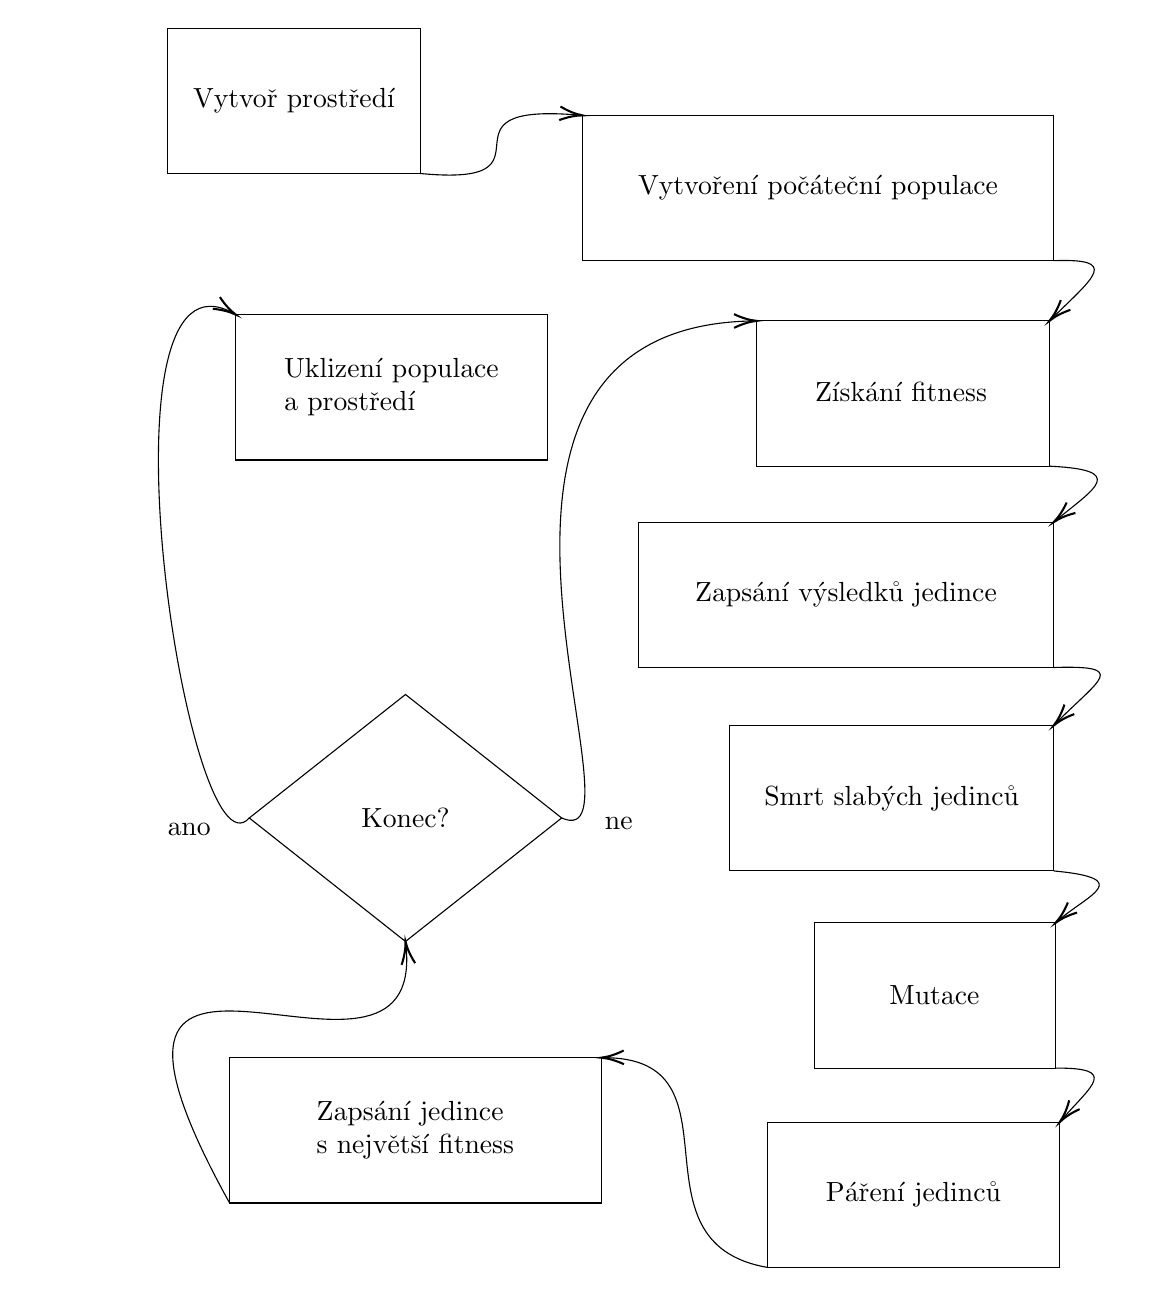
\begin{tikzpicture}[x=0.75pt,y=0.75pt,yscale=-1,xscale=1]
%uncomment if require: \path (0,644); %set diagram left start at 0, and has height of 644

%Flowchart: Process [id:dp06859388190835625] 
\draw   (11.5,18) -- (133.5,18) -- (133.5,88) -- (11.5,88) -- cycle ;
%Flowchart: Process [id:dp10980223482219675] 
\draw   (211.5,60) -- (438.5,60) -- (438.5,130) -- (211.5,130) -- cycle ;
%Flowchart: Process [id:dp00003710769396580993] 
\draw   (295.5,159) -- (436.5,159) -- (436.5,229) -- (295.5,229) -- cycle ;
%Flowchart: Process [id:dp4515117371988475] 
\draw   (238.5,256) -- (438.5,256) -- (438.5,326) -- (238.5,326) -- cycle ;
%Flowchart: Process [id:dp8901958980154814] 
\draw   (41.5,514) -- (220.5,514) -- (220.5,584) -- (41.5,584) -- cycle ;
%Flowchart: Process [id:dp9010826621566526] 
\draw   (282.5,354) -- (438.5,354) -- (438.5,424) -- (282.5,424) -- cycle ;
%Flowchart: Process [id:dp9622612195765325] 
\draw   (323.5,449) -- (439.5,449) -- (439.5,519) -- (323.5,519) -- cycle ;
%Flowchart: Process [id:dp7332866580581863] 
\draw   (300.5,545) -- (441.5,545) -- (441.5,615) -- (300.5,615) -- cycle ;
%Flowchart: Process [id:dp640384971132772] 
\draw   (44.5,156) -- (194.5,156) -- (194.5,226) -- (44.5,226) -- cycle ;
%Flowchart: Decision [id:dp5675790897815314] 
\draw   (126.25,339) -- (201.5,398.5) -- (126.25,458) -- (51,398.5) -- cycle ;
%Curve Lines [id:da44022975898520644] 
\draw    (201.5,398.5) .. controls (248,419) and (123,160) .. (295.5,159) ;
\draw [shift={(295.5,159)}, rotate = 539.6700000000001] [color={rgb, 255:red, 0; green, 0; blue, 0 }  ][line width=0.75]    (10.93,-3.29) .. controls (6.95,-1.4) and (3.31,-0.3) .. (0,0) .. controls (3.31,0.3) and (6.95,1.4) .. (10.93,3.29)   ;

%Curve Lines [id:da6241920896486743] 
\draw    (51,398.5) .. controls (21.15,431.66) and (-26.52,116.01) .. (43.44,155.38) ;
\draw [shift={(44.5,156)}, rotate = 211.12] [color={rgb, 255:red, 0; green, 0; blue, 0 }  ][line width=0.75]    (10.93,-3.29) .. controls (6.95,-1.4) and (3.31,-0.3) .. (0,0) .. controls (3.31,0.3) and (6.95,1.4) .. (10.93,3.29)   ;

%Curve Lines [id:da9023317836537514] 
\draw    (438.5,130) .. controls (470.35,128.85) and (458.5,137.47) .. (437.78,157.74) ;
\draw [shift={(436.5,159)}, rotate = 315.44] [color={rgb, 255:red, 0; green, 0; blue, 0 }  ][line width=0.75]    (10.93,-3.29) .. controls (6.95,-1.4) and (3.31,-0.3) .. (0,0) .. controls (3.31,0.3) and (6.95,1.4) .. (10.93,3.29)   ;

%Curve Lines [id:da11792313080682315] 
\draw    (436.5,229) .. controls (474.04,230.78) and (458.82,239.38) .. (439.96,254.8) ;
\draw [shift={(438.5,256)}, rotate = 320.33000000000004] [color={rgb, 255:red, 0; green, 0; blue, 0 }  ][line width=0.75]    (10.93,-3.29) .. controls (6.95,-1.4) and (3.31,-0.3) .. (0,0) .. controls (3.31,0.3) and (6.95,1.4) .. (10.93,3.29)   ;

%Curve Lines [id:da4726701559889561] 
\draw    (438.5,326) .. controls (475.25,324.85) and (460.62,331.55) .. (439.78,352.69) ;
\draw [shift={(438.5,354)}, rotate = 314.12] [color={rgb, 255:red, 0; green, 0; blue, 0 }  ][line width=0.75]    (10.93,-3.29) .. controls (6.95,-1.4) and (3.31,-0.3) .. (0,0) .. controls (3.31,0.3) and (6.95,1.4) .. (10.93,3.29)   ;

%Curve Lines [id:da2609603507608811] 
\draw    (438.5,424) .. controls (477.79,427.71) and (455.44,435.35) .. (440.83,447.83) ;
\draw [shift={(439.5,449)}, rotate = 317.75] [color={rgb, 255:red, 0; green, 0; blue, 0 }  ][line width=0.75]    (10.93,-3.29) .. controls (6.95,-1.4) and (3.31,-0.3) .. (0,0) .. controls (3.31,0.3) and (6.95,1.4) .. (10.93,3.29)   ;

%Curve Lines [id:da5702021903783518] 
\draw    (300.5,615) .. controls (231.35,602.89) and (291.39,513.73) .. (221.56,513.99) ;
\draw [shift={(220.5,514)}, rotate = 359.06] [color={rgb, 255:red, 0; green, 0; blue, 0 }  ][line width=0.75]    (10.93,-3.29) .. controls (6.95,-1.4) and (3.31,-0.3) .. (0,0) .. controls (3.31,0.3) and (6.95,1.4) .. (10.93,3.29)   ;

%Curve Lines [id:da1534096137301475] 
\draw    (41.5,584) .. controls (-55.51,408.71) and (137.06,555.35) .. (126.43,459.46) ;
\draw [shift={(126.25,458)}, rotate = 442.65] [color={rgb, 255:red, 0; green, 0; blue, 0 }  ][line width=0.75]    (10.93,-3.29) .. controls (6.95,-1.4) and (3.31,-0.3) .. (0,0) .. controls (3.31,0.3) and (6.95,1.4) .. (10.93,3.29)   ;

%Curve Lines [id:da6747434737872118] 
\draw    (439.5,519) .. controls (470.21,518.83) and (456.72,527.38) .. (442.59,543.73) ;
\draw [shift={(441.5,545)}, rotate = 310.18] [color={rgb, 255:red, 0; green, 0; blue, 0 }  ][line width=0.75]    (10.93,-3.29) .. controls (6.95,-1.4) and (3.31,-0.3) .. (0,0) .. controls (3.31,0.3) and (6.95,1.4) .. (10.93,3.29)   ;

%Curve Lines [id:da6714775938597657] 
\draw    (133.5,88) .. controls (204.64,94.79) and (134.71,53.25) .. (210.35,59.9) ;
\draw [shift={(211.5,60)}, rotate = 185.29] [color={rgb, 255:red, 0; green, 0; blue, 0 }  ][line width=0.75]    (10.93,-3.29) .. controls (6.95,-1.4) and (3.31,-0.3) .. (0,0) .. controls (3.31,0.3) and (6.95,1.4) .. (10.93,3.29)   ;


% Text Node
\draw (72.5,53) node  [align=left] {Vytvoř prostředí};
% Text Node
\draw (325,95) node  [align=left] {Vytvoření počáteční populace};
% Text Node
\draw (365,193) node  [align=left] {Získání fitness};
% Text Node
\draw (360.5,389) node  [align=left] {Smrt slabých jedinců};
% Text Node
\draw (381.09,484) node  [align=left] {Mutace};
% Text Node
\draw (371,580) node  [align=left] {Páření jedinců};
% Text Node
\draw (126.25,398.5) node  [align=left] {Konec?};
% Text Node
\draw (119.5,191) node  [align=left] {Uklizení populace\\a prostředí};
% Text Node
\draw (131,549) node  [align=left] {Zapsání jedince \\s největší fitness};
% Text Node
\draw (338.5,291) node  [align=left] {Zapsání výsledků jedince};
% Text Node
\draw (22,404) node  [align=left] {ano};
% Text Node
\draw (229,401) node  [align=left] {ne};


\end{tikzpicture}
\end{center}









































  
    
\end{document}
